\section{Testing the algorithm on LHCb data}

%Training machine learning algorithms on simulated data assumes that the simulation contains the same patterns as found in real physics.%
%Training machine learning algorithms on simulated data assumes that the simulation is a good approximation of real world physics.
%Although the performance of trained models can be evaluated on data that was not used for training, 

%A necessary step in developing any algorithm is to check whether this algorithm works in scenarios that it is intended for.
%The trained model in this thesis is intended to distinguish $B_d$ from $B_s$ mesons in $pp$-collisions independent of the decay channel.
%Additionally, the model is intended to classify processes of the physical world rather than the simulations it is trained on.
%Consequently, the final step of this thesis is testing the model on LHCb run 2 data of the decay $B^0 \rightarrow J/\psi + K_\text{S}$.
%This decay channel contains both the $B_d$ and $B_s$ mesons and the data 

Although the developed model of this thesis is intended to distinguish $B_d$ from $B_s$ mesons in $pp$-collisions independent of the decay channel, it is trained only on simulated data containing the decay channels $B_d \rightarrow J/\psi \, K^*$ and $B_s \rightarrow D^+_s \, \pi^-$.
Consequently, the trained model must be evaluated on LHCb data of some other decay channel.
Chosen here are the decays $B_d \text{ or } B_s \rightarrow J/\psi \, K^0_\text{S}$.
The dataset used here contains LHCb data from the years 2016, 2017 and 2018 that has been selected for both mentioned decays using similar selection criteria. 

Since this dataset originates from a real measurement rather than a simulation, the data contains a significant amount of background events.
In order to be able to fit the $B_s$ resonance, the amount of background events is reduced.
The procedure used for background reduction is based on the work-in-progress measurement of $\sin(2\beta)$ in $B^0\rightarrow J/\psi \, K^0_\text{S}$ decays with run 2 data, and is explained here only very briefly.

A few types of background are reduced manually.
One source of such background events is the misidentification of $\Lambda^0 \rightarrow p^+ \, \pi^-$ decays as $K^0_\text{S} \rightarrow \pi^+ \, \pi^-$.
To reduce this type of background, events are rejected if the reconstructed invariant mass of the $K^0_\text{S}$~candidate is in the region  of the $\Lambda^0$~mass (\qtyrange{1095}{1140}{\MeV}) and $\text{Prob}_p > \num{0.10}$ is required. 
Misidentified backgrounds from $B \rightarrow J/\psi \, K^*$ decays are rejected by requiring that the kaon candidate has a lifetime longer than $\qty{0.5}{\pico\second}$.
Finally, a cut $\chi^2(\text{fit})<\num{5.0}$ is applied. %TODO: mention features before explanation %TODO: after the BDT

To reduce all other types of combinatorial background, a BDT is trained.
Again, the BDT is implemented in Python using the library XGBoost \cite{xgboost}.
For this, events of the mentioned dataset with a reconstructed signal~$B$ mass larger than $\qty{5450}{\MeV}$ are used as background events, and simulated events of the decay $B_d \rightarrow J/\psi \, K^0_\text{S}$ are used as signal events.
The BDT has a maximum tree depth of 2, is trained at a learning rate of $0.3$ and consists of 2000 estimators.
A ROC AUC score of $0.989$ is achieved on test data and the corresponding ROC curve is shown in \autoref{fig:BKG_BDT_ROC}.
With this, events are classified as background events if the BDT output is smaller than $\num{0.5}$.

\begin{table}
    \centering
    \caption{List of all features used to train the BDT for the distinction between signal and background events.}
    \label{tab:BKG_BDT_features}
    \begin{tabular}{c c}
        \toprule
        feature & feature \\
        \midrule
        IP$(B^0)$                   & $p_\text{T}(\pi^+)$ \\% "B_IP_OWNPV","piplus_PT"
        IP$(J/\psi)$                & $p_\text{T}(\pi^-)$ \\% "Jpsi_IP_OWNPV","piminus_PT"
        IP$(K^0_\text{S})$          & $p_\text{T}(K^0_\text{S})$ \\% "KS0_IP_OWNPV","KS0_PT"
        IP$(\mu^+)$                 & $\eta(B^0)$ \\% "muplus_IP_OWNPV","B_LOKI_ETA"
        IP$(\mu^-)$                 & $\eta(K^0_\text{S})$ \\% "muminus_IP_OWNPV","KS0_LOKI_ETA"
        FD$(K^0_\text{S})$    & $p_z(K^0_\text{S})$ \\% "KS0_FD_OWNPV","KS0_PZ"
        $\chi^2(\text{fit})$  & \\% "B_LOKI_DTF_CHI2NDOF",
        \bottomrule
    \end{tabular}
\end{table}

The features used by the BDT are listed in \autoref{tab:BKG_BDT_features} and describe the signal $B$ and its decay particles.
The symbols inside the brackets represent the corresponding particle in the signal decay.
IP$(x)$ is the impact parameter to the production vertex of particle $x$.
$p_\text{T}(x)$ is the transversal momentum of particle $x$.
$\eta(x)$ is the pseudorapidity of particle $x$.
$p_z(x)$ is the momentum of particle $x$ along the $z$-axis.
FD$(x)$ is the flight distance from the production vertex to the decay vertex of particle $x$.
Finally, $\chi^2(\text{fit})$ is the $\chi^2$ corresponding to the reconstruction of the entire signal decay.

\begin{figure}
    \centering
    \begin{subfigure}{0.5\textwidth}
        \centering
        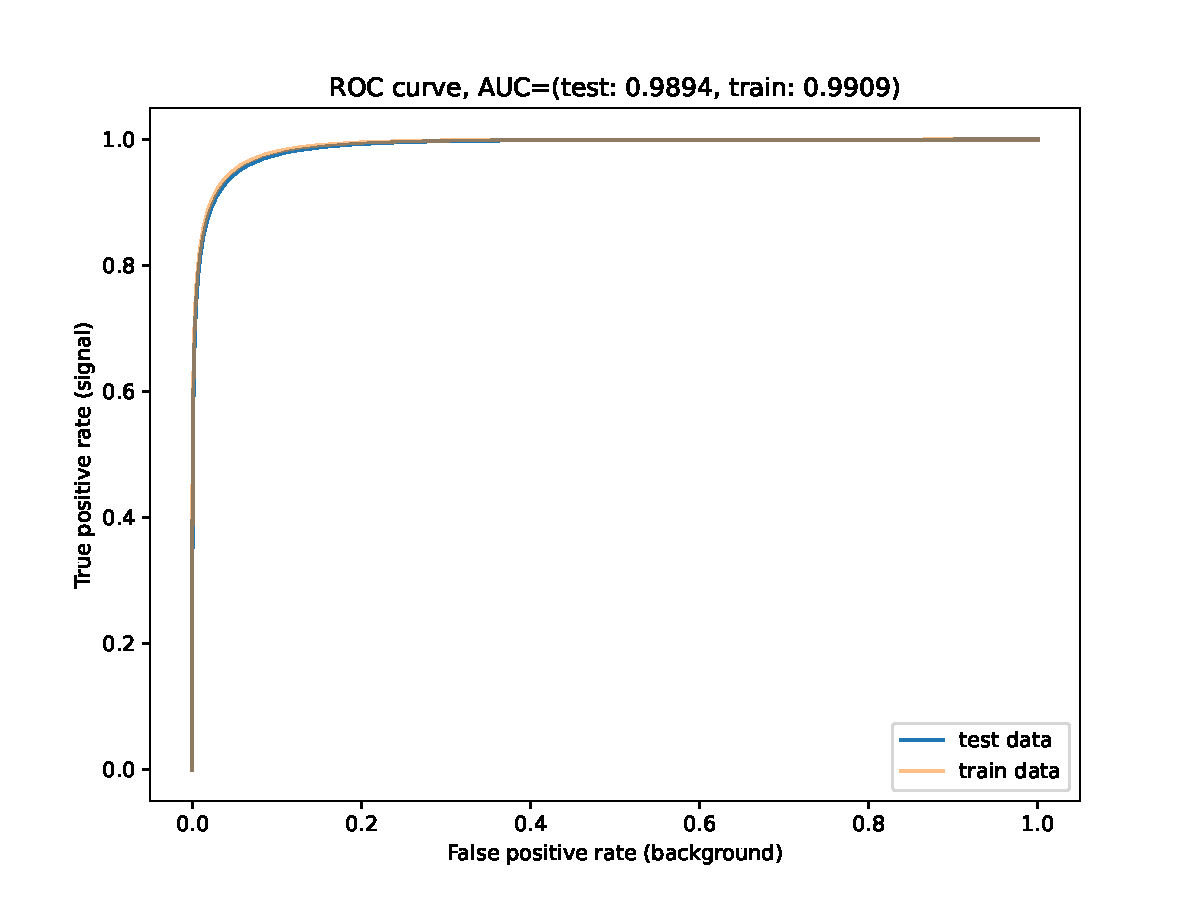
\includegraphics[width=\textwidth]{images/BKG_BDT_ROC.pdf}
        \caption{ROC curve of the BDT}
        \label{fig:BKG_BDT_ROC}
    \end{subfigure}%
    \begin{subfigure}{0.5\textwidth}
        \centering
        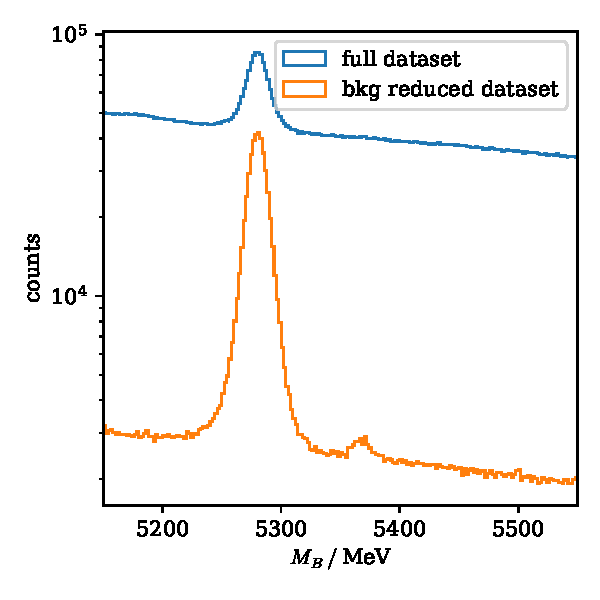
\includegraphics[width=\textwidth]{images/BKG_reduced.pdf}
        \caption{Distribution of the signal~$B$ mass}
        \label{fig:BKG_reduced}
    \end{subfigure}%
    \caption{The left figure shows the ROC curve achieved by the BDT for background identification. The right figure shows the distribution of the reconstructed signal~$B$ mass before and after reducing the background with the BDT and the manual cuts.}
    \label{fig:BKG_eval}
\end{figure}

\autoref{fig:BKG_reduced} shows the distribution of the reconstructed signal~$B$ mass before and after reducing the background with the BDT and the manual cuts.
After reducing the background, the trained model for the signal~$B$ classification is applied on the data to calculate $\text{Prob}_{B_s}$.
To estimate the performance of this prediction, an alternative method to estimate the amount of $B_d$ and $B_s$ mesons is needed.
The chosen procedure is to do a least squares fit on the $B$ mass distribution and estimate the counts of events by integrating each component of the fitted function.

In the following function definitions every variable except $M_B$ is a parameter that has to be fitted.
The $B$ mass distribution found in the data can be approximated by a function
\begin{equation*}
    F(M_B) = N_\text{bkg} \cdot F_\text{bkg}(M_B) + N_{B_d} \cdot F_{B_d}(M_B) + N_{B_s} \cdot F_{B_s}(M_B)
\end{equation*}
that is split into three components.
The first component $F_\text{bkg}$ describes the combinatorial background with 
\begin{align*}
    F_\text{bkg}(M_B) = \exp(-\lambda \cdot M_B) \, .
\end{align*}
The second component $F_{B_d}$ describes the events containing a $B_d$ meson and the third component $F_{B_s}$ describes the events containing a $B_s$ meson.
Both $F_{B_d}$ and $F_{B_s}$ use the same function
\begin{align*}
    F_B(M_B) = &f_1 \cdot f_2 \cdot F_\text{CB}\left(\frac{M_B-\mu}{\sigma_1}, \beta_1, m_1\right) \\
                    &+ (1-f_1) \cdot f_2 \cdot F_\text{CB}\left(-\frac{M_B-\mu}{\sigma_2}, \beta_2, m_2\right) \\
                    &+ (1-f_1) \cdot (1-f_2) \cdot F_\text{gauss}\left(M_B,\mu,\sigma_3\right) \, ,
\end{align*}
with the same parameters except $\mu_{B_s} = \mu_{B_d} + (M_{B_s}-M_{B_d})$.
$M_{B_d}=\qty{5279.65}{\MeV}$ is the mass of $B_d$ mesons and $M_{B_s}=\qty{5366.88}{\MeV}$ is the mass of $B_s$ mesons \cite{pdg}.
\begin{equation*}
    F_\text{CB}(x,\beta,m) = 
     \begin{cases}
         N \cdot \exp(-\frac{x^2}{2}) & \text{for } x > -\beta \\
         N \cdot \left(\frac{m}{|\beta|}\right)^m \cdot \exp\left(-\frac{\beta^2}{2}\right) \cdot \left(\frac{m}{|b|}-|b| - x\right)^{-m} & \text{for } x \leq -\beta
     \end{cases}
\end{equation*}
is called a Crystal Ball distribution and
\begin{equation*}
    F_\text{gauss}\left(x,\mu,\sigma\right) = \frac{1}{\sqrt{2}\pi} \cdot \exp\left(-\frac{1}{2}\left(\frac{x-\mu}{\sigma}\right)^2\right)
\end{equation*}
is called a normal distribution.

All the following fits are done using the library \enquote{iminuit}\cite{iminuit}.
First, a fit is done on the simulated data of the $B_d$ peak to fix the parameters $f_1,f_2,\beta_1,\beta_2,m_1$ and $m_2$ for all the following fits. 
This fit is shown in \autoref{fig:fit_mc}.
Then, for 100 values of $x$ between 0 and 1, a selection with $\text{Prob}_{B_s} \leq x$ and a selection with $\text{Prob}_{B_s} \geq x$ is made.
A fit is done on each acquired $B$ mass distribution and the counts
\begin{align*}
    n_{B_d} &= \int_{-\infty}^{\infty} N_{B_d} \cdot F_{B_d}(M_B) \, \symup{d}M_B \:\:\text{ and} \\
    n_{B_s} &= \int_{-\infty}^{\infty} N_{B_s} \cdot F_{B_s}(M_B) \, \symup{d}M_B
\end{align*}
are calculated numerically.
One of those fitted distributions is shown in \autoref{fig:fit_example}.

\begin{figure}
    \centering
    \begin{subfigure}{0.5\textwidth}
        \centering
        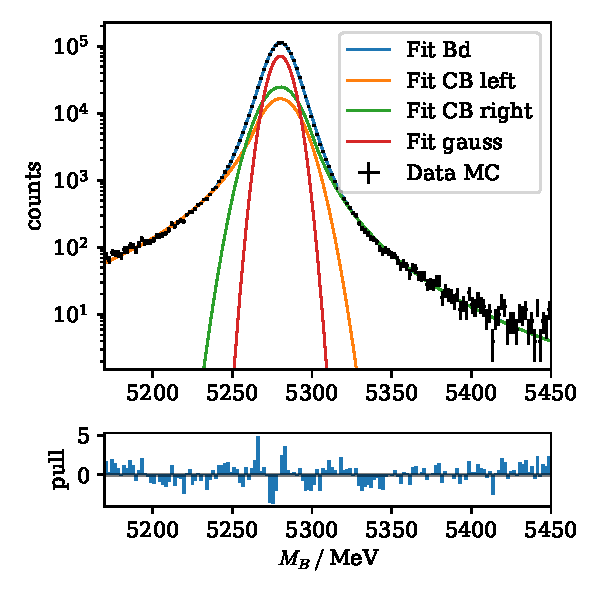
\includegraphics[width=\textwidth]{images/fit_mc.pdf}
        \caption{Fit of the $B_d$ peak}
        \label{fig:fit_mc}
    \end{subfigure}%
    \begin{subfigure}{0.5\textwidth}
        \centering
        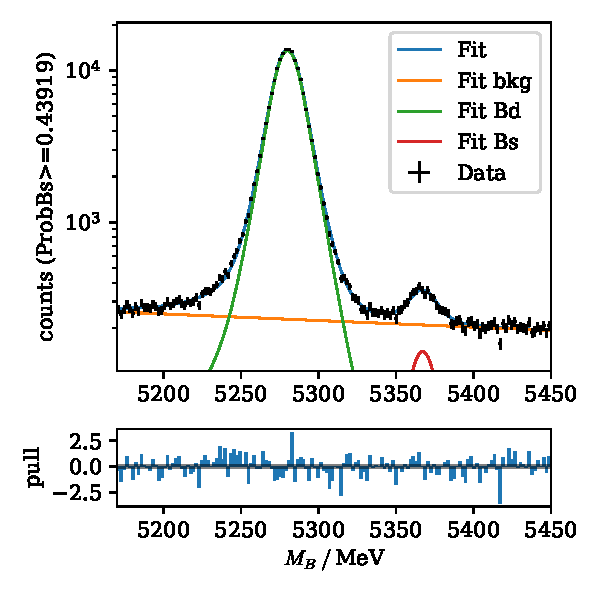
\includegraphics[width=\textwidth]{images/fit_example.pdf}
        \caption{Example fit of a data selection}
        \label{fig:fit_example}
    \end{subfigure}%
    \caption{The left figure shows a fit on simulated data of the $B_d$ peak. The right figure shows a fit of the $B$ mass distribution with the selection $\text{Prob}_{B_s} \geq 0.43919$. Both figures also show a pull distribution between the data points and the fit.}
\end{figure}

To estimate how good the trained model of this thesis can distinguish $B_d$ and $B_s$ mesons, the ratio $n_{B_s}/n_{B_d}$ is plotted by the cut value $x$ for selections with $\text{Prob}_{B_s} \geq x$. 
This is shown in \autoref{fig:data_ratio}.
The expected value without any achieved separation is 
\begin{equation*}
    \frac{\text{BR}(B_s \rightarrow J/\psi + K^0_\text{S})}{\text{BR}(B_d \rightarrow J/\psi + K^0_\text{S})} \cdot 
    f_s/f_d(\qty{13}{\TeV}) = \num{0.0109\pm0.0010} \, .
\end{equation*}
Where the branching ratios are $\text{BR}(B_s \rightarrow J/\psi + K^0_\text{S}) = \num{4.37\pm0.16e-4}$ and $\text{BR}(B_d \rightarrow J/\psi + K^0_\text{S}) = \num{1.88\pm0.15e-5}$ \cite{pdg}, and $f_s/f_d(\qty{13}{\TeV}) = \num{0.2539\pm0.0079}$ is the ratio of the $B^0_s$ and $B^0$ fragmentation fractions in $pp$-collisions at $\qty{13}{\TeV}$ collision energy \cite{fsfd}.
%Where BR stands for branching fraction and $\frac{f_s}{f_d}(\qty{13}{\TeV})$ is the ratio of the $B^0_s$ and $B^0$ fragmentation fractions in $pp$-collisions at $\qty{13}{\TeV}$.

Another approach to show the achieved separation, is to plot a curve similar to a ROC curve. 
For each selection, the estimated efficiencies
\begin{align*}
    \varepsilon_{B_d} &= \frac{n_{B_d}(x)}{n_{B_d}(\text{no cut})} \: \: \text{ and} \\
    \varepsilon_{B_s} &= \frac{n_{B_s}(x)}{n_{B_s}(\text{no cut})}
\end{align*}
are calculated. Shown in \autoref{fig:data_roc} is the plot of $\varepsilon_{B_d}$ against $\varepsilon_{B_s}$.
%Without any achieved separation, the plot would show a straight line from $(0,0)$ to $(1,1)$.
Similar to a ROC curve, a diagonal line from $(0,0)$ to $(1,1)$ is the expectation without any achieved separation.
Compared to the achieved ROC curve on the simulated data shown in \autoref{fig:B_ROC}, a substantially weaker separation is achieved on the LHCb data.

\begin{figure}
    \centering
    \begin{subfigure}{0.5\textwidth}
        \centering
        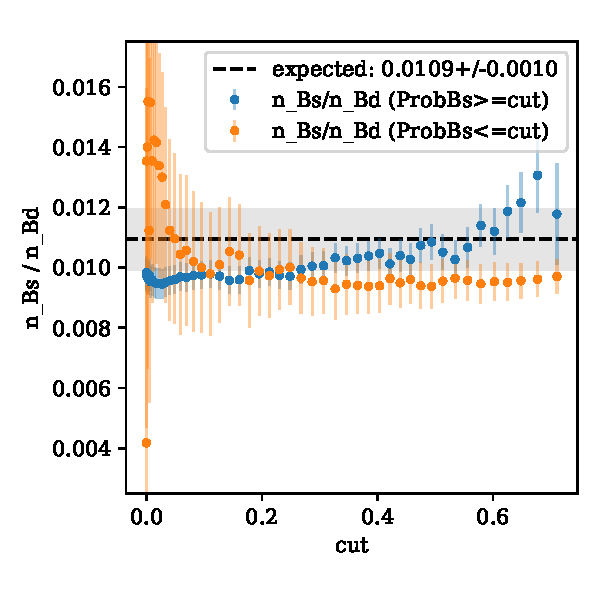
\includegraphics[width=\textwidth]{images/data_ratio.pdf}
        \caption{Ratio $n_{B_s}/n_{B_d}$ by cut value}
        \label{fig:data_ratio}
    \end{subfigure}%
    \begin{subfigure}{0.5\textwidth}
        \centering
        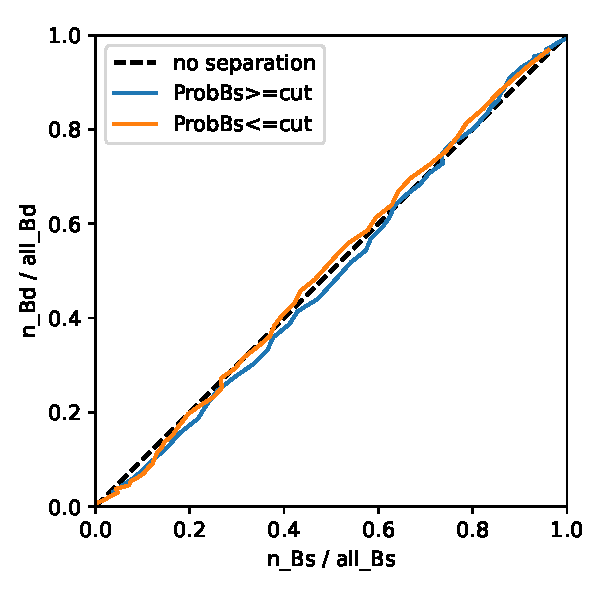
\includegraphics[width=\textwidth]{images/data_roc.pdf}
        \caption{similar to a ROC curve}
        \label{fig:data_roc}
    \end{subfigure}%
    \caption{The left figure shows the estimated ratio $n_{B_s}/n_{B_d}$. Here, it is important to note that selections with $\text{Prob}_{B_s} \leq x$ on small $x$ have a very small $B_s$ peak, which makes the interpretation of these ratios almost impossible. The right figure shows the estimated efficiencies $\varepsilon_{B_d}$ agains $\varepsilon_{B_s}$. In both figures, selections with $\text{Prob}_{B_s} \geq x$ are shown in blue and selections with $\text{Prob}_{B_s} \leq x$ are shown in orange.}
\end{figure}


